\documentclass[11pt]{article}

\author{Math 123}
\date{Due February 3, 2023 by 5pm} 
\title{Homework 1}

\newcommand{\cc}{\mathbb{C}}
\newcommand{\ff}{\mathbb{F}}
\renewcommand{\gg}{\mathbb{G}}
\newcommand{\nn}{\mathbb{N}}
\newcommand{\qq}{\mathbb{Q}}
\newcommand{\rr}{\mathbb{R}}
\newcommand{\zz}{\mathbb{Z}}

\usepackage{graphicx,xypic}
\usepackage{amsthm}
\usepackage{amsmath,amssymb}
\usepackage{amsfonts}
\usepackage{xcolor}
\usepackage[margin=1in]{geometry}
\usepackage[shortlabels]{enumitem}
\newtheorem{problem}{Problem}
\renewcommand*{\proofname}{{\color{blue}Solution}}

% tikz
\usepackage{tikz}
\usetikzlibrary{intersections, angles, quotes, positioning}
\usetikzlibrary{arrows.meta}
\usepackage{pgfplots}
\pgfplotsset{compat=1.13}


\tikzset{
	force/.style={thick, {Circle[length=2pt]}-stealth, shorten <=-1pt}
}

% quiver style
\usepackage{tikz-cd}
% `calc` is necessary to draw curved arrows.
\usetikzlibrary{calc}
% `pathmorphing` is necessary to draw squiggly arrows.
\usetikzlibrary{decorations.pathmorphing}

% A TikZ style for curved arrows of a fixed height, due to AndréC.
\tikzset{curve/.style={settings={#1},to path={(\tikztostart)
					.. controls ($(\tikztostart)!\pv{pos}!(\tikztotarget)!\pv{height}!270:(\tikztotarget)$)
					and ($(\tikztostart)!1-\pv{pos}!(\tikztotarget)!\pv{height}!270:(\tikztotarget)$)
					.. (\tikztotarget)\tikztonodes}},
	settings/.code={\tikzset{quiver/.cd,#1}
			\def\pv##1{\pgfkeysvalueof{/tikz/quiver/##1}}},
	quiver/.cd,pos/.initial=0.35,height/.initial=0}

% TikZ arrowhead/tail styles.
\tikzset{tail reversed/.code={\pgfsetarrowsstart{tikzcd to}}}
\tikzset{2tail/.code={\pgfsetarrowsstart{Implies[reversed]}}}
\tikzset{2tail reversed/.code={\pgfsetarrowsstart{Implies}}}
% TikZ arrow styles.
\tikzset{no body/.style={/tikz/dash pattern=on 0 off 1mm}}


\usepackage{fancyhdr}
\pagestyle{fancy}
\rhead{Math 123, Homework 1}

\setlength{\parindent}{0pt}
\setlength{\parskip}{1.25ex}


\begin{document}

\maketitle

% You are required to put your name here:
{\bf\Large Name: George Chemmala} 


\vspace{.3in}
Topics covered: graph, subgraph, cycle, path, vertex degrees, 

Instructions: 
\begin{itemize}
\item This assignment must be submitted on Grade scope by the due date. Grade scope Entry Code: RZ277D. 
\item If you collaborate with other students (which is encouraged!), please mention this near the corresponding problems. 
\item If you are stuck, please ask for help (from me, a TA, a classmate).  
\end{itemize}

\pagebreak 


\begin{problem}
Prove that the graph below is isomorphic to the Petersen graph.\footnote{Hint: label the graph.}
\begin{center}
    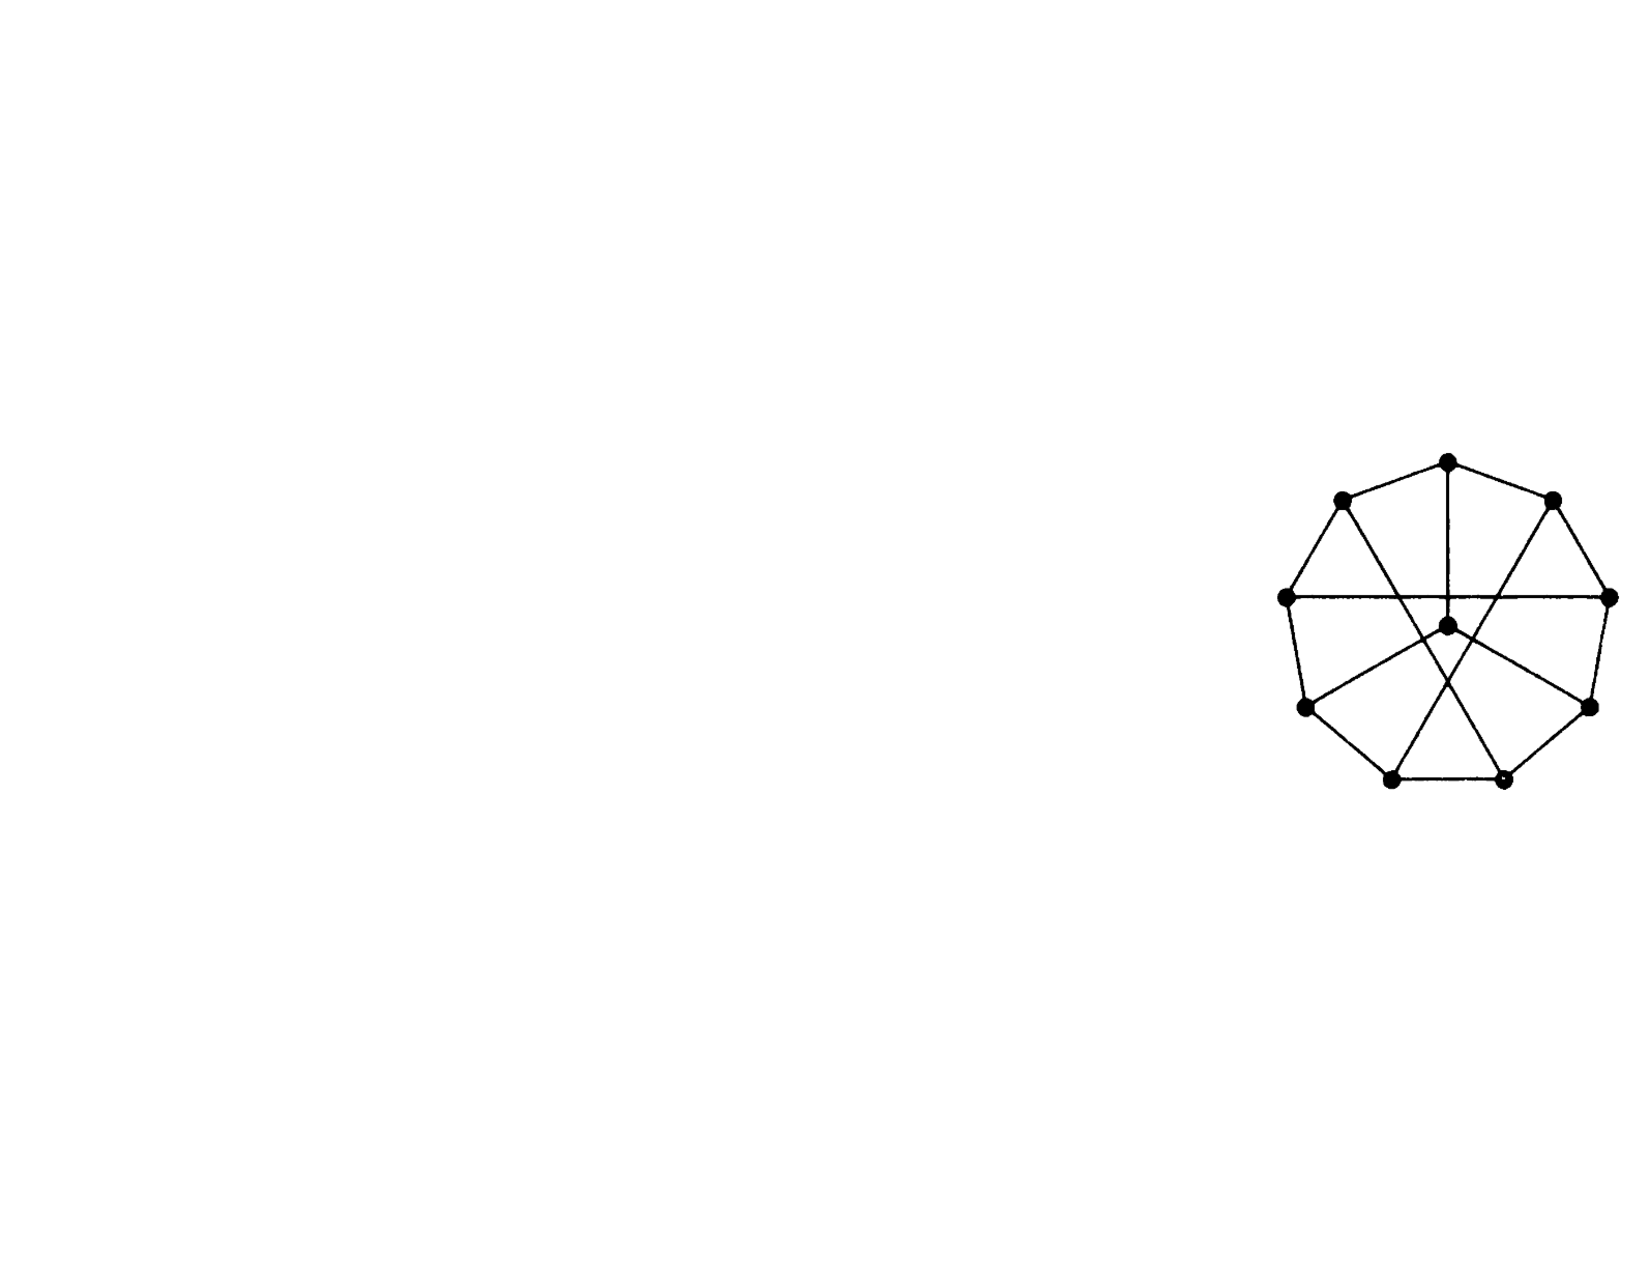
\includegraphics[scale=.4]{petersen.pdf}
\end{center}
\end{problem}

\begin{proof}
I tried to best replicate the graph using tikz:
% https://q.uiver.app/?q=WzAsMTAsWzAsMSwiMTQiXSxbMCwyLCIzMiJdLFs0LDEsIjI1Il0sWzQsMiwiMTMiXSxbMSwwLCIzNSJdLFszLDAsIjM0Il0sWzIsMCwiMTIiXSxbMSwzLCIxNSJdLFszLDMsIjI0Il0sWzIsMSwiNDUiXSxbMCwxLCIiLDIseyJzdHlsZSI6eyJoZWFkIjp7Im5hbWUiOiJub25lIn19fV0sWzIsMywiIiwyLHsic3R5bGUiOnsiaGVhZCI6eyJuYW1lIjoibm9uZSJ9fX1dLFsyLDUsIiIsMCx7InN0eWxlIjp7ImhlYWQiOnsibmFtZSI6Im5vbmUifX19XSxbNCw2LCIiLDAseyJzdHlsZSI6eyJoZWFkIjp7Im5hbWUiOiJub25lIn19fV0sWzUsNiwiIiwxLHsic3R5bGUiOnsiaGVhZCI6eyJuYW1lIjoibm9uZSJ9fX1dLFsxLDcsIiIsMix7InN0eWxlIjp7ImhlYWQiOnsibmFtZSI6Im5vbmUifX19XSxbMyw4LCIiLDIseyJzdHlsZSI6eyJoZWFkIjp7Im5hbWUiOiJub25lIn19fV0sWzcsOCwiIiwxLHsic3R5bGUiOnsiaGVhZCI6eyJuYW1lIjoibm9uZSJ9fX1dLFs4LDQsIiIsMSx7ImN1cnZlIjotNCwic3R5bGUiOnsiaGVhZCI6eyJuYW1lIjoibm9uZSJ9fX1dLFs1LDcsIiIsMSx7ImN1cnZlIjotNCwic3R5bGUiOnsiaGVhZCI6eyJuYW1lIjoibm9uZSJ9fX1dLFswLDIsIiIsMSx7ImN1cnZlIjotMiwic3R5bGUiOnsiaGVhZCI6eyJuYW1lIjoibm9uZSJ9fX1dLFs5LDEsIiIsMSx7InN0eWxlIjp7ImhlYWQiOnsibmFtZSI6Im5vbmUifX19XSxbOSwzLCIiLDEseyJzdHlsZSI6eyJoZWFkIjp7Im5hbWUiOiJub25lIn19fV0sWzksNiwiIiwxLHsic3R5bGUiOnsiaGVhZCI6eyJuYW1lIjoibm9uZSJ9fX1dLFs0LDAsIiIsMix7InN0eWxlIjp7ImhlYWQiOnsibmFtZSI6Im5vbmUifX19XV0=
\[\begin{tikzcd}
	& 35 & 12 & 34 \\
	14 && 45 && 25 \\
	32 &&&& 13 \\
	& 15 && 24
	\arrow[no head, from=2-1, to=3-1]
	\arrow[no head, from=2-5, to=3-5]
	\arrow[no head, from=2-5, to=1-4]
	\arrow[no head, from=1-2, to=1-3]
	\arrow[no head, from=1-4, to=1-3]
	\arrow[no head, from=3-1, to=4-2]
	\arrow[no head, from=3-5, to=4-4]
	\arrow[no head, from=4-2, to=4-4]
	\arrow[curve={height=-24pt}, no head, from=4-4, to=1-2]
	\arrow[curve={height=-24pt}, no head, from=1-4, to=4-2]
	\arrow[curve={height=-12pt}, no head, from=2-1, to=2-5]
	\arrow[no head, from=2-3, to=3-1]
	\arrow[no head, from=2-3, to=3-5]
	\arrow[no head, from=2-3, to=1-3]
	\arrow[no head, from=1-2, to=2-1]
\end{tikzcd}\]

This labeling of the graph fits the definition of the Petersen graph.
\end{proof}


\begin{problem}
How many cycles of length $n$ are there in the complete graph $K_n$?
\end{problem}

\begin{proof}
We can define a cycle as a list of vertices (like how we label walks). For example, \(v_1\ldots v_n\) There are \(n!\) different ways to order this list, but we must divide this by \(n\) (permutations are isomorphic since a cycle can start from \(n\) starting points) and by \(2\) since the permutations are isomorphic backwards and forwards. Therefore, there are \(\frac{(n-1)!}{2}\) cycles of length \(n\) 
\end{proof}

\begin{problem}
Define the hypercube graph $Q_k$ as the graph with a vertex for each tuple $(a_1,\ldots,a_k)$ with coordinates $a_i\in\{0,1\}$ and with an edge between $(a_1,\ldots,a_k)$ and $(b_1,\ldots,b_k)$ if they differ in exactly one coordinate.\footnote{Suggestion: Draw $Q_k$ for $k=2$ and $k=3$.} 
\begin{enumerate}[(a)]
\item Prove that two $4$-cycles in $Q_k$ are either disjoint, intersect in a single vertex, or intersect in a single edge.
\item Let $K_{2,3}$ be the complete bipartite graph with $2$ red vertices, $3$ blue vertices, and all possible edges between red and blue vertices. Prove that $K_{2,3}$ is not a subgraph of any hypercube $Q_k$. 
\end{enumerate} 
\end{problem}

\begin{proof}
\begin{enumerate}[(a)]
	\item The following will show that cases where the 4-cycles are disjoint, intersect in a single vertex, or intersect in a single edge are possible and then show intersection beyond 2 points is not possible:
	
	Example of existence of 2 disjoint 4-cycles: 

	\(\{(0000), (0001), (0011), (0010)\}\) and \(\{(0101), (0111), (0100), (0110)\}\)

	Example of existence of 2 4-cycles that intersect at a single vertex: 

	\(\{(0000), (0001), (0011), (0010)\}\) and \(\{(0000), (0100), (1000), (1100)\}\)

	Example of existence of 2 4-cycles that intersect in a single edge: 

	\(\{(0000), (0001), (0011), (0010)\}\) and \(\{(0000), (0010), (1000), (1010)\}\)

	Explanation of nonexistence 4-cycles that intersect at 3 vertices:

	For all 4-cycles the addition of all points must be equal to \((0 \ldots 0)\) in order to be closed cycles. For example, in the case of \(\{(0000), (0001), (0011), (0010)\}\), \((0 + 0 + 0 + 0, 0 + 0 + 0 + 0, 0 + 0 + 1 + 1, 0 + 1 + 1 + 0) = (0,2,2,0)=(0,0,0,0)\) Essentially, we are working in \(\zz_{2} \times \ldots \times \zz_{2}\). When we add 3 points in a cycle we get the 4th point since \( p_1 + p_2 + p_3 + p_4 = (0,0,0,0) \iff p_1 + p_2 + p_3 = -p_4 = p_4\) Therefore, if there were two 4-cycles that intersect at 3 vertices, they must be the same cycle - a contradiction.

	Explanation of nonexistence 4-cycles that intersect at more than 4 vertices:

	If the two 4-cycles intersect at 4 vertices they must be the same cycle - a contradiction. If they intersect at more than 4 vertices that is a contradiction with the condition that there are 4 vertices in 4-cycles

	\item In the last problem we showed that a 4-cycle in a hypercube graph cannot intersect another separate 4-cycle with 3 points. However, this is possible in \(K_{2,3}\):
	
	\(K_{2,3}\)
	% https://q.uiver.app/?q=WzAsNSxbMSwwLCJcXGJ1bGxldCJdLFswLDIsIlxcYnVsbGV0Il0sWzQsMiwiXFxidWxsZXQiXSxbMiwyLCJcXGJ1bGxldCJdLFszLDAsIlxcYnVsbGV0Il0sWzAsMSwiIiwwLHsic3R5bGUiOnsiYm9keSI6eyJuYW1lIjoiZGFzaGVkIn0sImhlYWQiOnsibmFtZSI6Im5vbmUifX19XSxbMCwyLCIiLDIseyJzdHlsZSI6eyJib2R5Ijp7Im5hbWUiOiJkYXNoZWQifSwiaGVhZCI6eyJuYW1lIjoibm9uZSJ9fX1dLFswLDMsIiIsMix7InN0eWxlIjp7ImJvZHkiOnsibmFtZSI6ImRhc2hlZCJ9LCJoZWFkIjp7Im5hbWUiOiJub25lIn19fV0sWzQsMSwiIiwyLHsic3R5bGUiOnsiYm9keSI6eyJuYW1lIjoiZGFzaGVkIn0sImhlYWQiOnsibmFtZSI6Im5vbmUifX19XSxbNCwzLCIiLDAseyJzdHlsZSI6eyJib2R5Ijp7Im5hbWUiOiJkYXNoZWQifSwiaGVhZCI6eyJuYW1lIjoibm9uZSJ9fX1dLFs0LDIsIiIsMCx7InN0eWxlIjp7ImJvZHkiOnsibmFtZSI6ImRhc2hlZCJ9LCJoZWFkIjp7Im5hbWUiOiJub25lIn19fV1d
\[\begin{tikzcd}
	& \bullet && \bullet \\
	\\
	\bullet && \bullet && \bullet
	\arrow[dashed, no head, from=1-2, to=3-1]
	\arrow[dashed, no head, from=1-2, to=3-5]
	\arrow[dashed, no head, from=1-2, to=3-3]
	\arrow[dashed, no head, from=1-4, to=3-1]
	\arrow[dashed, no head, from=1-4, to=3-3]
	\arrow[dashed, no head, from=1-4, to=3-5]
\end{tikzcd}\]
	
	1st 4-cycle in \(K_{2,3}\)
% https://q.uiver.app/?q=WzAsNSxbMSwwLCJhIl0sWzAsMiwieCJdLFs0LDIsInoiXSxbMiwyLCJ5Il0sWzMsMCwiYiJdLFswLDEsIiIsMCx7InN0eWxlIjp7ImhlYWQiOnsibmFtZSI6Im5vbmUifX19XSxbMCwyLCIiLDIseyJzdHlsZSI6eyJib2R5Ijp7Im5hbWUiOiJkYXNoZWQifSwiaGVhZCI6eyJuYW1lIjoibm9uZSJ9fX1dLFswLDMsIiIsMix7InN0eWxlIjp7ImhlYWQiOnsibmFtZSI6Im5vbmUifX19XSxbNCwxLCIiLDIseyJzdHlsZSI6eyJoZWFkIjp7Im5hbWUiOiJub25lIn19fV0sWzQsMywiIiwwLHsic3R5bGUiOnsiaGVhZCI6eyJuYW1lIjoibm9uZSJ9fX1dLFs0LDIsIiIsMCx7InN0eWxlIjp7ImJvZHkiOnsibmFtZSI6ImRhc2hlZCJ9LCJoZWFkIjp7Im5hbWUiOiJub25lIn19fV1d
\[\begin{tikzcd}
	& a && b \\
	\\
	x && y && z
	\arrow[no head, from=1-2, to=3-1]
	\arrow[dashed, no head, from=1-2, to=3-5]
	\arrow[no head, from=1-2, to=3-3]
	\arrow[no head, from=1-4, to=3-1]
	\arrow[no head, from=1-4, to=3-3]
	\arrow[dashed, no head, from=1-4, to=3-5]
\end{tikzcd}\]

	2nd 4-cycle in \(K_{2,3}\)
% https://q.uiver.app/?q=WzAsNSxbMSwwLCJhIl0sWzAsMiwieCJdLFs0LDIsInoiXSxbMiwyLCJ5Il0sWzMsMCwiYiJdLFswLDEsIiIsMCx7InN0eWxlIjp7ImJvZHkiOnsibmFtZSI6ImRhc2hlZCJ9LCJoZWFkIjp7Im5hbWUiOiJub25lIn19fV0sWzAsMiwiIiwyLHsic3R5bGUiOnsiaGVhZCI6eyJuYW1lIjoibm9uZSJ9fX1dLFswLDMsIiIsMix7InN0eWxlIjp7ImhlYWQiOnsibmFtZSI6Im5vbmUifX19XSxbNCwxLCIiLDIseyJzdHlsZSI6eyJib2R5Ijp7Im5hbWUiOiJkYXNoZWQifSwiaGVhZCI6eyJuYW1lIjoibm9uZSJ9fX1dLFs0LDMsIiIsMCx7InN0eWxlIjp7ImhlYWQiOnsibmFtZSI6Im5vbmUifX19XSxbNCwyLCIiLDAseyJzdHlsZSI6eyJoZWFkIjp7Im5hbWUiOiJub25lIn19fV1d
\[\begin{tikzcd}
	& a && b \\
	\\
	x && y && z
	\arrow[dashed, no head, from=1-2, to=3-1]
	\arrow[no head, from=1-2, to=3-5]
	\arrow[no head, from=1-2, to=3-3]
	\arrow[dashed, no head, from=1-4, to=3-1]
	\arrow[no head, from=1-4, to=3-3]
	\arrow[no head, from=1-4, to=3-5]
\end{tikzcd}\]

Both 4-cycles share \(a\), \(b\), \(y\), but are not the same 4-cycle  

\end{enumerate}
\end{proof}

\begin{problem}
For a graph $G=(V,E)$, the complement of $G$ is the graph $\bar G=(V,\bar E)$, where $\{u,v\}\in\bar E$ if and only if $\{u,v\}\notin E$. Prove or disprove: If $G$ and $H$ are isomorphic, then the complements $\bar G$ and $\bar H$ are also isomorphic. 
\end{problem}

\begin{proof}
For all edges in \(\widetilde{G}\), \(\widetilde{G}\) has an edge \(\iff \) \(G\) doesn't have an edge \(\iff\) \(H\) doesn't have an edge \(\iff\) \(\widetilde{H}\) has an edge. Therefore, for all edges in \(\widetilde{G}\),  \(\widetilde{G}\) has an edge \(\iff\) \(\widetilde{H}\) has an edge.
\end{proof}


\begin{problem}
\begin{enumerate}[(a)]
\item Determine the complement of the graphs $P_3$ and $P_4$. (Recall that $P_n$ is the path with $n$ vertices. It has $n-1$ edges.)
\item We say that $G$ is self-complementary if $G$ is isomorphic $\bar G$. Prove that if $G$ is self-complementary with $n$ vertices, then either $n$ is divisible by $4$ or $n-1$ is divisible by $4$. \footnote{Hint: count edges}
\end{enumerate} 
In fact, whenever $n$ or $n-1$ is divisible by $4$, there is a self-complementary graph with $n$ vertices -- see the bonus problem below. 
\end{problem}

\begin{proof}
\begin{enumerate}
    \item[(a)] \(\widetilde{P_3}\) \& \(\widetilde{P_4}\): 
    
    \(\widetilde{P_3}\) 
    % https://q.uiver.app/?q=WzAsMyxbMCwwLCJcXGJ1bGxldCJdLFs0LDAsIlxcYnVsbGV0Il0sWzIsMCwiXFxidWxsZXQiXSxbMCwxLCIiLDAseyJjdXJ2ZSI6LTMsInN0eWxlIjp7ImhlYWQiOnsibmFtZSI6Im5vbmUifX19XV0=
    \[\begin{tikzcd}
        \bullet && \bullet && \bullet
        \arrow[curve={height=-18pt}, no head, from=1-1, to=1-5]
    \end{tikzcd}\]

    \(\widetilde{P_4}\)
    % https://q.uiver.app/?q=WzAsNCxbMCwwLCJcXGJ1bGxldCJdLFs0LDAsIlxcYnVsbGV0Il0sWzIsMCwiXFxidWxsZXQiXSxbNSwwLCJcXGJ1bGxldCJdLFswLDEsIiIsMCx7ImN1cnZlIjotMywic3R5bGUiOnsiaGVhZCI6eyJuYW1lIjoibm9uZSJ9fX1dLFsyLDMsIiIsMCx7ImN1cnZlIjoyLCJzdHlsZSI6eyJoZWFkIjp7Im5hbWUiOiJub25lIn19fV0sWzMsMCwiIiwwLHsiY3VydmUiOi01LCJzdHlsZSI6eyJoZWFkIjp7Im5hbWUiOiJub25lIn19fV1d
\[\begin{tikzcd}
	\bullet && \bullet && \bullet & \bullet
	\arrow[curve={height=-18pt}, no head, from=1-1, to=1-5]
	\arrow[curve={height=12pt}, no head, from=1-3, to=1-6]
	\arrow[curve={height=-30pt}, no head, from=1-6, to=1-1]
\end{tikzcd}\]
\end{enumerate}

    \item[(b)] The sum of the number of edges of a graph and it's complement has to be the number of edges in \(K_n\) i.e \({n \choose 2} = n(n-1)/2\) and if \(G\) is self-complementary \(G\), it's complement, \(\widetilde{G}\), must have the same number of edges; therefore \(G\) and \(\widetilde{G}\) have \(n(n-1)/4\) edges. Since the number of edges is an integer, \(G\) can only be self-complementary when \(n(n-1)/4\) is an integer, which is equivalent to either \(n\) or \((n-1)\) being divisible by 4 since only either \(n\) or \((n-1)\)  could divide 4 (\(n\) and \(n-1\) are consecutive). 
\end{proof}


\begin{problem}Prove that the Petersen graph has no cycles of length $3$ or $4$. \footnote{Hint: use the definition of Petersen graph given in class.} 
\end{problem}

\begin{proof}
We will suppose the cycles are possible and show how they lead to contradictions of the definition of the Petersen graph:

Suppose there exists a 3-cycle then this would require:
% https://q.uiver.app/?q=WzAsMyxbMCwwLCJhYiJdLFsxLDAsImNkIl0sWzAsMSwiZWYiXSxbMCwxLCIiLDAseyJzdHlsZSI6eyJoZWFkIjp7Im5hbWUiOiJub25lIn19fV0sWzAsMiwiIiwyLHsic3R5bGUiOnsiaGVhZCI6eyJuYW1lIjoibm9uZSJ9fX1dLFsyLDEsIiIsMix7InN0eWxlIjp7ImhlYWQiOnsibmFtZSI6Im5vbmUifX19XV0=
\[\begin{tikzcd}
	ab & cd \\
	ef
	\arrow[no head, from=1-1, to=1-2]
	\arrow[no head, from=1-1, to=2-1]
	\arrow[no head, from=2-1, to=1-2]
\end{tikzcd}\]

Where \(a\), \(b\), \(c\), \(d\), \(e\), and \(f\) are all different, to satisfy one of the Petersen graph definition conditions, but there is a contradiction with the Petersen graph definition condition that are only 5 different choices (there can be no \(f\) ).

Suppose there exists a 4-cycle:

There must be 2 vertices which are disjoint from 1 vertex:
% https://q.uiver.app/?q=WzAsMyxbMCwwLCJhYiJdLFsxLDAsImNkIl0sWzAsMSwiZGUiXSxbMCwxLCIiLDEseyJzdHlsZSI6eyJoZWFkIjp7Im5hbWUiOiJub25lIn19fV0sWzAsMiwiIiwxLHsic3R5bGUiOnsiaGVhZCI6eyJuYW1lIjoibm9uZSJ9fX1dXQ==
\[\begin{tikzcd}
	ab & cd \\
	de
	\arrow[no head, from=1-1, to=1-2]
	\arrow[no head, from=1-1, to=2-1]
\end{tikzcd}\]

There must be one repeated value between the two non-connected vertices since there are only 2 choices up to isomorphism from choosing between \(c\)  \(d\), and \(e\) (we are limited to 5 different choices, \(a\), \(b\), \(c\), \(d\), and \(e\), by definition of the Petersen graph) 

When we add another vertex, it also needs to be disjoint from the 2 vertices; therefore, it cannot be \(b\), \(c\), and \(e\) forcing it to choose the remaining \(a\) and \(b\), but this is a contradiction.

% https://q.uiver.app/?q=WzAsNCxbMCwwLCJhYiJdLFsxLDAsImNkIl0sWzAsMSwiZGUiXSxbMSwxLCJhYiJdLFswLDEsIiIsMSx7InN0eWxlIjp7ImhlYWQiOnsibmFtZSI6Im5vbmUifX19XSxbMCwyLCIiLDEseyJzdHlsZSI6eyJoZWFkIjp7Im5hbWUiOiJub25lIn19fV0sWzIsMywiIiwxLHsic3R5bGUiOnsiaGVhZCI6eyJuYW1lIjoibm9uZSJ9fX1dLFsxLDMsIiIsMSx7InN0eWxlIjp7ImhlYWQiOnsibmFtZSI6Im5vbmUifX19XV0=
\[\begin{tikzcd}
	ab & cd \\
	de & ab
	\arrow[no head, from=1-1, to=1-2]
	\arrow[no head, from=1-1, to=2-1]
	\arrow[no head, from=2-1, to=2-2]
	\arrow[no head, from=1-2, to=2-2]
\end{tikzcd}\]

\end{proof}

\begin{problem}[Bonus]
Let $G,H$ be a self-complementary graphs, and assume $G$ has with $4k$ vertices. Construct a self-complementary graph obtained by taking the union of $G$ and $H$ and adding some edges.\footnote{Hint: How does the degree of even/odd vertices of $G$ change after taking the complement?} Deduce that if either $n$ or $n-1$ is divisible by $4$, then there is a self-complementary graph with $n$ vertices. 
\end{problem}

\begin{proof}
I believe an algorithm for doing this would be to connect all vertices of \(H\) to all vertices in \(G\) that have even degree. Unfortunately, I have not yet found a proof of this but playing around adjacency matrices seems to suggest this (e.g, \(P_4 + P_4\) results in the same odd/even degree switch while \(P_4 + C_5\) results is all the degrees having the same parity). We have shown in problem 5 that \(P_4\) is self-complementary and \(C_5\) is also self-complementary. Therefore, we can create any graph of \(n\), where either \(n\)  or \(n-1\) is divisible by \(4\), using a combination of \(P_4\) and \(C_5\) with the aforementioned algorithm.  
\end{proof}


\end{document}